\documentclass{beamer}

\usepackage{graphicx,hyperref,udesc,url}
\usepackage[utf8]{inputenc}
\usepackage[T1]{fontenc}
\usepackage{booktabs}
%\usepackage[portugues]{babel}
\usepackage{amssymb}
\usepackage[utf8]{inputenc}
\usepackage[brazil]{babel}
\usepackage{csquotes}
\usepackage{listings}
\usepackage{amsmath}
\usepackage{amsthm}
\usepackage{mathtools}
\usepackage{verbatim}
%\usepackage[table,xcdraw]{xcolor}
\usepackage{multirow}

\title[]{Otimizações para Motores de Jogos Através de Modelagem Orientada a Dados}

\author[Vinicius Bruch Zuchi]{
    Vinicius Bruch Zuchi\\\medskip
    {\small \url{vinicius.b.zuchi@gmail.com}\\}}

\institute[UDESC]{
    Departamento de Ci\^encia da Computa\c{c}\~ao \\
    Centro de Ci\^encias e Tecnol\'ogicas\\
Universidade do Estado de Santa Catarina}

\begin{document}

\begin{frame}
    \titlepage
\end{frame}

\begin{frame}
    \frametitle{Sum\'ario}
    \tableofcontents
\end{frame}

\section{Recapitulando}

\frame{\tableofcontents[currentsection]}

\begin{frame}[t]{Problema}
\end{frame}

\begin{frame}[t]{Motor de Jogos}
\end{frame}

\begin{frame}[t]{Como Solucionar}
\end{frame}

\section{Modelagem Orientada a Dados}

\frame{\tableofcontents[currentsection]}

\begin{frame}[t]{Origem e Popularização}
\end{frame}

\begin{frame}[t]{Principais Ideias}
\end{frame}

\begin{frame}[t]{Como Armazenar os Dados}
\end{frame}

\begin{frame}[t]{Branching e Prefetching}
\end{frame}

\section{O Trabalho Desenvolvido}

\frame{\tableofcontents[currentsection]}

\begin{frame}[t]{Motivação}
\end{frame}

\begin{frame}[t]{Aplicações Desenvolvidas}
\end{frame}

\begin{frame}[t]{Etapas de Conversão}
\end{frame}

\begin{frame}[t]{Diferenças Entre as Abordagens}
\end{frame}

\begin{frame}[t]{Método de Renderização}
\end{frame}

\begin{frame}[t]{Método de Atualização}
\end{frame}

\begin{frame}[t]{Detecção de Colisões}
\end{frame}

\section{Análises e Resultados}

\frame{\tableofcontents[currentsection]}

\begin{frame}[t]{Cenários Desenvolvidos}
\end{frame}

\begin{frame}[t]{Problema A: Médias}
\end{frame}

\begin{frame}[t]{Problema A: Draw}
\end{frame}

\begin{frame}[t]{Problema A: Update}
\end{frame}

\begin{frame}[t]{Problema A: Collision}
\end{frame}

\begin{frame}[t]{Problema B: Médias}
\end{frame}

\begin{frame}[t]{Problema B: Draw}
\end{frame}

\begin{frame}[t]{Problema B: Update}
\end{frame}

\begin{frame}[t]{Problema B: Collision}
\end{frame}

\section{Conclusão}

\frame{\tableofcontents[currentsection]}

\begin{frame}[t]{Diferença de MOO e MOD}
    \begin{figure}
    \centering
        \begin{minipage}[b]{0.35\textwidth}
            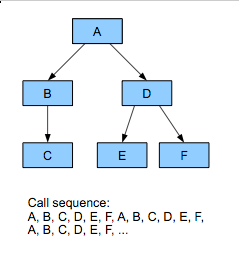
\includegraphics[width=\textwidth]{figuras/objectreadingorder}
        \end{minipage}
        \begin{minipage}[b]{0.35\textwidth}
            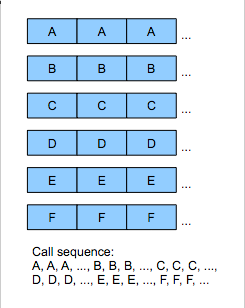
\includegraphics[width=\textwidth]{figuras/dodreadingorder}
        \end{minipage}
        %\par\medskip
        %Disponível em: <http://gamesfromwithin.com/data-oriented-design>. Acesso em: 27/05/2017.
        %\label{oodvsdod}
    \end{figure}
\end{frame}

\begin{frame}{Fim}
    \centering
    \LARGE{That's All Folks!}
\end{frame}

\end{document}
